\documentclass{exam}
\usepackage[utf8]{inputenc}
\usepackage{color}
\usepackage{amsmath}
\usepackage[english]{babel}
\usepackage{comment}
\usepackage{graphicx}
\usepackage{wrapfig}
\usepackage{caption}
\usepackage{subcaption}
\usepackage[siunitx]{circuitikz}
\newcommand{\splitcell}[2][c]{%
  \begin{tabular}[c]{@{}c@{}}\strut#2\strut\end{tabular}%
}
\usepackage{natbib}
\usepackage{listings}
\usepackage{xparse}
\usepackage{hyperref}
\usepackage{float}
\usepackage{tcolorbox}

\NewDocumentCommand{\codeword}{v}{%
\texttt{\textcolor{blue}{#1}}%
}
\usepackage{pgfplots}
\pgfplotsset{compat = newest}
\usepackage{chngcntr}
\counterwithin{table}{section}
\counterwithin{figure}{section}

\usepackage{listings}
\usepackage{xcolor}

\definecolor{codegreen}{rgb}{0,0.6,0}
\definecolor{codegray}{rgb}{0.5,0.5,0.5}
\definecolor{codepurple}{rgb}{0.58,0,0.82}
\definecolor{backcolour}{rgb}{0.95,0.95,0.92}

\lstdefinestyle{mystyle}{
    backgroundcolor=\color{backcolour},   
    commentstyle=\color{codegreen},
    keywordstyle=\color{magenta},
    numberstyle=\tiny\color{codegray},
    stringstyle=\color{codepurple},
    basicstyle=\ttfamily\footnotesize,
    breakatwhitespace=false,         
    breaklines=true,                 
    captionpos=b,                    
    keepspaces=true,                 
    numbers=left,                    
    numbersep=5pt,                  
    showspaces=false,                
    showstringspaces=false,
    showtabs=false,                  
    tabsize=2
}

\lstset{style=mystyle}

\begin{document}

\newcommand{\Exjobbsnummer}[1]{
	\begin{tikzpicture}[overlay, remember picture]
		\path (current page.north east) ++(-1,-1) node[below left] {{\small #1}};
	\end{tikzpicture}
}

\newcommand{\Examensjobbspoang}[1]{
	\begin{tikzpicture}[overlay, remember picture]
		\path (current page.north east) ++(-1,-1.5) node[below left] {{\normalsize \scshape Examensarbete #1 HP}};
	\end{tikzpicture}
}

\newcommand{\datum}[1]{
	\begin{tikzpicture}[overlay, remember picture]
		\path (current page.north east) ++(-1,-2.0) node[below left] {{\normalsize #1}};
	\end{tikzpicture}}

\newcommand{\storlitentitel}[2]{
\center
\rule[0.2cm]{13cm}{0.1cm}
{ \huge \bfseries #1}\\[0.4cm] % Title of your document
{\Large \slshape #2}\\[0.4cm]
\rule[0.2cm]{13cm}{0.1cm}\\[3cm]

}

\newcommand{\Namn}[2]{
	\begin{minipage}{0.5\textwidth}
		\normalsize
		\centering
		#1 \textsc{#2}\\
	\end{minipage}\\
}

\newcommand{\LoggaSwe}{
	\textsc{\Huge Internet Performance \\[0.3cm] and Troubleshooting Lab}\\[0.7cm]
	
\includegraphics[scale=.06]{polito_logo_2021_blu.jpg}\\[1.5cm]
}

\newcommand{\LoggaEng}{
	\textsc{\Huge Uppsala University}\\[0.7cm]
	\includegraphics[scale=.1]{Uppsala_University_seal_svg.png}\\[0.5cm]
}

% -----------------------------------------------
%           HÄR BÖRJAR TITELSIDAN
%------------------------------------------------
\begin{titlepage}

	\center

	%-------------------------------------------------
	%	INFORMATION ATT FYLLA I
	%-------------------------------------------------
	\Exjobbsnummer{Academic Year 2023/2024}
	%\datum{2021/2022}

	\LoggaSwe
	% \LoggaEng - Byt till engelska

	\storlitentitel{\\Report V}{Video Streaming}

	\Large Group 3\\
	\Namn{Brendon Mendicino}{(s317639)}
	\Namn{Alessandro Ciullo}{(s310023)}
	\Namn{Davide Colaiacomo}{(s313372)}

	\vfill

\end{titlepage}
\pagebreak

\section{Introduction}
\subsection{Network Configuration}
\begin{figure}[H]
    \centering
    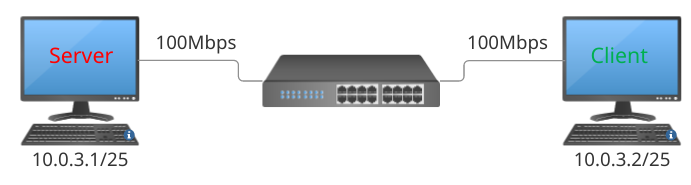
\includegraphics[width=0.70\linewidth]{network_topology.png}
    \caption{Network Topology}
    \label{fig:enter-label}
\end{figure}

All tests but the \verb|asymmetric channel| ones were performed with both channels at 100Mbps \textit{bit-rate} and with a 200ms \textit{delay} both at the server and the client.

\subsection{Streaming configuration}
The objective of this laboratory is to develop knowledge and awareness regarding the functioning of video streaming. The tool we used to create our testing environment is \verb|VideoLanClient (VLC)|, a software that, contrary to what the name might suggest, is able to set up a server and a client for streaming. \verb|VLC| offers three streaming protocols: 
\begin{itemize}
    \item \textbf{UDP}: this protocol offers a fast but unreliable way of streaming in which the server sends the stream encapsulated in a \textbf{UDP} header to a designed host.
    \item \textbf{RTP}:This protocol offers additional functionality, like detection of packet loss and out-of-order delivery, over the \textbf{UDP} protocol.
    \item \textbf{HTTP}: In this streaming schema, \textbf{HTTP} is encapsulated in \textbf{TCP}, offering reliability and the choice to request a file by sending an \verb|HTTP GET| to the server; these functionalities are paid in term of performance. 
\end{itemize}

The test video we used during the experiments is \textit{jellyfish-50-mbps-hd-h264}, an mkv 1080p video with a bit-rate of 50Mbps. 

\section{Packet Size and Inter-packet Gap}
\subsection{Packet Size}
During the streaming videos are encapsulated in a container format of choice (multiplexing). In our case we picked the \verb|MPEG-TS| container that can be used to stream with all type of transport protocol. This container is made of unit of 188 bytes and adds information about timing needed by the client for synchronization. 

Since UDP is an unreliable packet oriented transport protocol, VLC sends only udp packets with a payload of 1316 bytes, exactly 7 \verb|MPEG-TS| units (entire packet is 1358 bytes and 1370 with RTP 12 bytes header) and so packet size appears constant during all the transmission. 

When HTTP is used the behavior of the payload length is different. Since TCP is a reliable stream oriented protocol, sending a payload containing exactly a multiple of the container format unit does not give additional advantages: everything will reach the other host and the \verb|PUSH| flag is added when a multiple is reached. The push packets, that needs to reach a MPEG-TS unit multiple, creates variability in packet length when HTTP is used.
The differences between the two protocol can be observed in figure \ref{fig:plain-len}

\begin{figure}[H]
    \centering
    \includegraphics[width=0.4\linewidth]{plain-len.pdf}
    \caption{Packet length with different transport protocols}
    \label{fig:plain-len}
\end{figure}

\subsection{Inter Packet Gap}

The interpacket gap can be observed in the following figure \ref{fig:plain-gap}.

\begin{figure}[H]
    \centering
    \includegraphics[width=0.4\linewidth]{plain-gap.pdf}
    \caption{inter packet gap with different transport protocol}
    \label{fig:plain-gap}
\end{figure}

The first thing that catches our eyes is the significant variability of the value we are analysing for the HTTP protocol compared to the more stable UDP (and RTP) where the Inter-packet gap stays in the order of hunder of microseconds. This is caused by the way flow control and TCP socket scheduling is performed in the kernel: we can in fact observe in Wireshark a long cluster of TCP segments sent to the client (that fill the receiving window)  followed by the corresponding cluster of ACKs sent to the server; this phenomenon creates those spikes in the HTTP graph. 

The second thing we want to address are the bigger gap (nearly a second) that both protocol shows. Those spikes are caused by the end of the video loop iteration: when the streaming is resetted for a significant amount of time no packets are sent from the server to the client in all protocols.

\section{Plain video streaming}
The first set of tests we conducted was related to the streaming of the plain video, without further elaboration; we decided to observe what happens when we perform the streaming relying on the \textbf{HTTP} protocol (which is based on \textbf{TCP}), on \textbf{UDP} and \textbf{RTP} (which is based on \textbf{UDP}).

\subsection{HTTP streaming}
For this first experiment with \textbf{HTTP}, we started an \textbf{HTTP} server that can receive \textbf{HTTP} requests, by means of the following command:
\begin{lstlisting}[language=bash]
vlc sample.mp4 --sout="#transcode{vcodec=h264, acodec=mpga,vb=800,ab=8}:std{access=http, mux=ts, http-host=10.0.3.1, port=8080}" --loop
\end{lstlisting}
On the other side, we run the \textbf{HTTP} client in order to open an \textbf{HTTP} connection with the aforementioned server by means of the following command: 
\begin{lstlisting}[language=bash]
vlc http://10.0.3.1:8080 --extraintf rc --rc-host=:1200 --loop
\end{lstlisting}
Observing figure~\ref{fig:plain_http_client}, we can notice that the bit-rate maintains itself on an average of 50 Mbps, with some downfalls happening at a periodical delay of about 30 seconds; this is due to the restart of the connection, that happens each time the video is completed (\textbf{HTTP} requires the opening of a new connection when the video is requested to be streamed again). From the point of view of the perceived quality of the video, we noticed that, in the plain video scenario, this is the strongest one thanks to the reliability of the \textbf{TCP} underlying protocol; this can also be sustained by the number of packet losses, which can be seen to equal 5 before being set back to 0 when the streaming starts over.

\subsection{UDP streaming}
For the next experiment, we changed the transmitting protocol used and tested \textbf{UDP}; in this case, we started a \textbf{UDP} server with the command:
\begin{lstlisting}[language=bash]
vlc sample.mp4 --sout="#transcode{vcodec=h264, acodec=mpga,vb=800,ab=8}:std{access=udp, mux=ts, dst=10.0.3.2, port=1234}" --loop
\end{lstlisting}
On the client side, we executed \textit{cvlc} in order to receive \textbf{UDP} data and play the received video with the command:
\begin{lstlisting}[language=bash]
vlc udp://:1234 --extraintf rc --rc-host=:1200 --loop
\end{lstlisting}
Observing figure~\ref{fig:plain_udp_client}, what we can see is that the streaming maintains itself at around 50 Mbps in a fairly stable way, but the real difference from the previous experiment with \textbf{HTTP} is that the perceived quality was much worse; this can be explained by the number of packet losses, that is much higher and goes over 30 by the time the test is completed. In general, this is a situation that could have been expected due to the \textbf{UDP} protocol \textit{best effort} policies, which do not guarantee any reliability.

\section{Transcoded video streaming}
During this test, the objective was to analyze the network behavior and stream performance when the video, before being streamed, is transcoded into a different format, more suitable to streaming purposes. HD videos can be transcoded between 3 and 9 Mbps (based of frame rate) without a perceptible loss of quality, reducing the burden on the connection from 50Mbps to the new bit rate, but paying with addition computing resources on server side.

During the following experiments we transcode the video to two different h264 output with bit rate of 5Mbps and 9Mbps in mp4 format. Since our PCs are not able to perform transcoding in real time we transcoded the video before the tests: we observed a lot of discontinuity in the video when transcoding was done on the fly. 

\subsection{HTTP streaming}
When the trans-coded video is streamed using http the first thing we observe is an average bandwidth consumption that matches the new bit rate. While the average network usage is what we expect there are big spikes of TCP traffic at the start of each loop iteration (from 30 to 100\% more than the video bit rate) as observable in figure \ref{fig:server_transcode_http_9000_lungo}. This could be caused by the new HTTP GET sent at the end of a video since on the first loop the spike is not present. 

We can theorize that the end of a loop iteration and the start of the new one overlaps for a small time frame. This creates also some synchronization problem between client and server since the video on the next iteration is displayed at screen only after circa 6-7 seconds. This behavior is not present in the original video stream, so we can think that this is correlated to the bit rate or the format or the video, only things that differs between the two experience: a major burden on the server or client made by the usage of a heavier bit rate could, surprisingly, create a more synchronized environment.


For what concerns the frame cumulative loss, as we can see from the graph \ref{fig:transcode_http_9000_frame} are 0, so the first 6-7 seconds of video that we are unable to see at screen are not reported (not even as discontinuities) by vlc. We can assume that the entire start of the streaming is effectively delayed.


\subsection{UDP stream}
By adopting udp for the streaming of the transcoded videos we can appreciate a improved QoS compared to the original video, and a burden on the network very similar to the video bit rate.

By observing the graph of cumulative loss in figure \ref{fig:transcode_udp_9000_frame} we can see how only 2 frames are lost over the duration of the experiment, a great improvement!
Similar results are obtained with both 5Mbps and 9Mbps streams.



\section{Impact of packet loss}
In this experience, we performed our test in an environment with an artificial percentage of packet loss set with the command:
\begin{lstlisting}
    tc qdisctc qdisc change dev eth0 root netem delay 200ms loss 0.1
\end{lstlisting}
We performed the tests with 0.1\% and 1\% loss probability and sending only the the 9Mbps video transcoded.

\subsection{HTTP stream}
With a loss probability of 1\% the video was never displayed: we can assume that the time needed to retransmit the lost packets was too big to perform a successful recovery, because the data received in the time lapse of a single frame was not enough to show the corresponding frame, also caused by the 400ms RTT. The input bit-rate of the stream was never higher than 2Mbps.

With a loss probability of 0.1\% we got a better Quality of Service. Nearly no frame was missing on the screen and the input bit-rate of the stream reached the expected value of 9Mbps as shown in figure \ref{fig:loss_http_9000_frame}.


We can assume that retransmissions are a lot more effective when the ploss percentage is 0.1\%.

\subsection{UDP stream}
With a loss probability of 1\% the video was never displayed but the input bit rate of the stream was higher than the corresponding http stream. 

With a loss probability of 0.1\% the video appeared at screen but with a lot of discontinuities and the input bit rate was a lot more unstable compared to the test done without ploss (shown in figure\ref{fig:loss_udp_9000_frame}).



\section{Impact on channel capability}
In this section, we are going to analyze what emerges when we try to perform the streaming of the same video, but with parallel connections happening on the same path of the streaming connection. To saturate the channel capacity, we used \texttt{iperf3} (with \textbf{TCP}) to generate more traffic on the same path and this affects differently with respect to the different streaming protocols. With \textbf{HTTP}, we tried two different setups: in the first one, \texttt{iperf3} is already exchanging data, in the second one we start the streaming first and then \texttt{iperf3}. We can see in figure~\ref{fig:http-iperf3} how \texttt{iperf3} takes the whole bandwidth of the channel and, when we start the streaming, the connection is not able to gain a lot of bit-rate, probably due to the \textit{TCP Congestion Control}. In the other case, we can see how the channel is shared more fairly between them, because the streaming already has half of the capacity; this is due to the fact that the server will have a downtime between when the video finishes and when it starts looping back and, as a consequence, during this downtime \texttt{iperf3} is able to regain all the lost bandwidth, and with a short video like ours the \textbf{TCP} connection of the streaming will never be able to cause enough losses to \texttt{iperf3} to share fairly the channel.

On the other hand, using \textbf{UDP} instead of \textbf{HTTP}, we expect that \texttt{iperf3} will not affect a lot the performance of the streaming; in fact, by looking at figure~\ref{fig:udp-iperf3}, we can see how the bandwidth of the \texttt{iperf3} connection is never able to reach the full capacity. The difference was also very noticeable from the streaming quality, as when using \textbf{HTTP} only one/two frames correctly displayed on screen, while with \textbf{UDP} we didn't see any noticeable difference from the standard case.

\begin{figure}[h]
    \centering
    \begin{subfigure}{0.45\textwidth}
        \centering
        \includegraphics[width=1\textwidth]{fotina5000_1iperf.pdf}
        \caption{\texttt{iperf3} (Purple)  with head start over HTTP streaming (5Mb/s) (Yellow)}
    \end{subfigure}
    \hfill
    \begin{subfigure}{0.45\textwidth}
        \centering
        \includegraphics[width=1\textwidth]{fotina5000_1stream.pdf}
        \caption{HTTP streaming (5Mb/s) (Yellow) with head start over \texttt{iperf3} (Purple)}
    \end{subfigure}
    \caption{Bit-rate of the \texttt{iperf3}  and the HTTP streaming connections.}
    \label{fig:http-iperf3}
\end{figure}

\begin{figure}
    \centering
    \includegraphics[width=0.5\linewidth]{fotina9000.pdf}    
    \caption{Bit-rate of UDP streaming (9Mb/s) (Yellow) and \texttt{iperf3} (Purple)}
    \label{fig:udp-iperf3}
\end{figure}

\section{Multicast}
What we also tried was to create a Multicast streaming connection inside our LAN (which is basically like a Broadcast connection for our purposes). With our previous approaches we can only establish a Unicast connection with a single host, but what would happen if we had more than one host to stream to? Our server will have to duplicate the connections, in the case of live trans-coding we expect to see a notable increase in the CPU usage of the server, because we will need to open two separate connections with two separate trans-coding happening at the same time, instead with a Multicast connection we can just send one packet and the router will send automatically the traffic to host subscribed to the Multicast group, this is very desirable because duplicating the a packet is less expensive than creating two separate trans-coding. On top of that Multicast an optimal choice in case of many users asking for a streaming service, the duplication of the packet is done by the Network infrastructure allowing also low-power devices to be able to stream live content to many clients.
\begin{figure}[h]
    \centering
    \begin{subfigure}{0.45\textwidth}
        \centering
        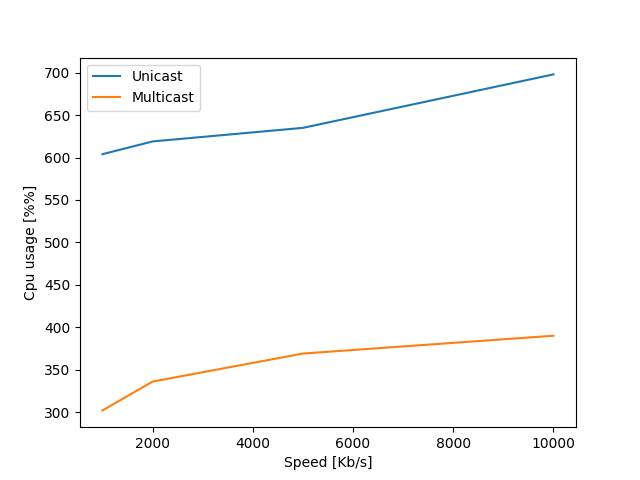
\includegraphics[width=1\textwidth]{uni-vs-multi-live.png}
        \caption{CPU usage during streaming with live trans-coding}
    \end{subfigure}
    \hfill
    \begin{subfigure}{0.45\textwidth}
        \centering
        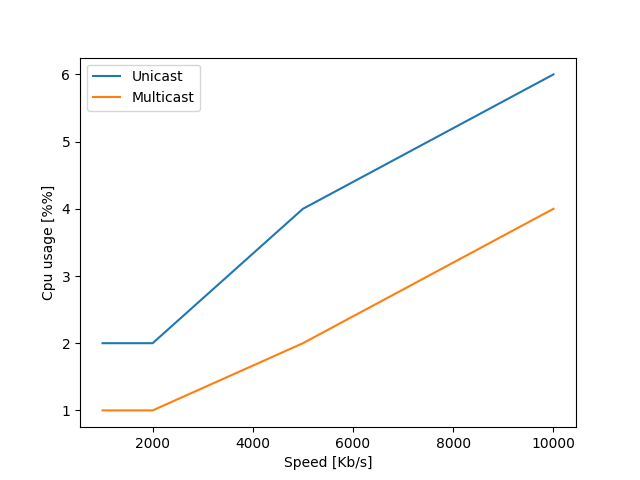
\includegraphics[width=1\textwidth]{uni-vs-multi-stored.png}
        \caption{CPU usage during streaming with stored trans-coding}
    \end{subfigure}
    \caption{CPU percentage measured over a period of 100 seconds.}
    \label{fig:cpu-usage}
\end{figure}
As we can see from the Figure~\ref{fig:cpu-usage} we used the following setup:
\begin{itemize}
\item [Unicast] two unicast connections opened.
\item [Multicast] one multicast connction opened.
\end{itemize}
It's easy to see that when we have more than one users, it would be way better to choose a Multicast connection over a Unicast one.

To create Multicast streaming with \texttt{vlc} we can use one the reserved addresses for IPv4 Multicast
\begin{lstlisting}[language=bash]
# Server
cvlc input --sout="#udp{mux=ts,dst=224.0.0.1,sdp=sap,name='TestStream'}"

# Client
vlc udp://@224.0.0.1
\end{lstlisting}
When writing the streaming parameters we use \texttt{sap} (\href{https://datatracker.ietf.org/doc/html/rfc2974}{Session Announcement Protocol}) that it is supposed provide the announcement of the Multicast session. The client simply listens to the Multicast session address to be able to visualize the stream.

\section{Streaming YouTube videos}
Using the \texttt{yt-dlp} (\href{https://github.com/yt-dlp/yt-dlp}{https://github.com/yt-dlp/yt-dlp}) utility it's possible to stream directly YouTube videos through or inside \texttt{vlc}. The first thing we can do is to stream the video directly to \texttt{vlc}
\begin{lstlisting}[language=bash]
yt-dlp -o - "https://www.youtube.com/watch?v=dQw4w9WgXcQ" | vlc -
\end{lstlisting}
In this way \texttt{vlc} is able to read the video directly from the \texttt{stdin} and display it to the screen, the \texttt{-o -} doesn't save the video in a folder but it directly sends it to \texttt{stdout}.

Using this technique we can only stream the YouTube video to our PC, and then take those data and stream it back using \texttt{vlc}.
\begin{lstlisting}[language=bash]
yt-dlp --hls-use-mpegts -o - "https://www.youtube.com/watch?v=dQw4w9WgXcQ" | cvlc - --sout="#udp{mux=ts,dst=224.0.0.1,sdp=sap,name='YoutubeSteaming'}"
\end{lstlisting}
The \texttt{--hls-use-mpegts} allows \texttt{yt-dlp} is used to start streaming the video as soon it gets the data without the need to download it fully first. This is usually used to re-stream YouTube Live Streaming.

\pagebreak
\section{Appendix}

\subsection{Plain Video Streaming}

\begin{figure}[H]
    \centering
    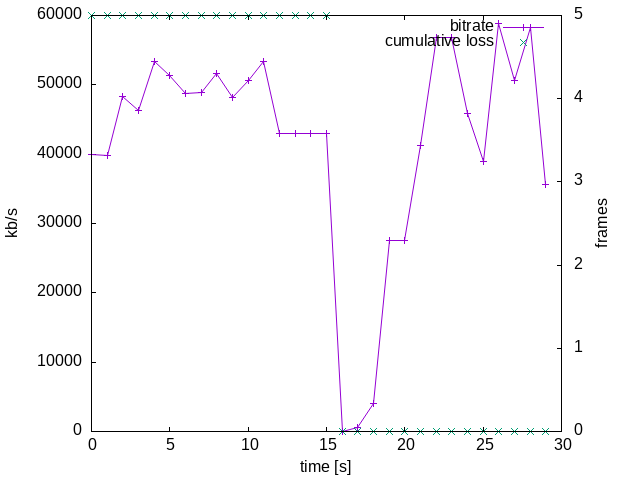
\includegraphics[width=0.5\linewidth]{plain_http_client.png}
    \caption{HTTP plain streaming - client}
    \label{fig:plain_http_client}
\end{figure}

\begin{figure}[H]
    \centering
    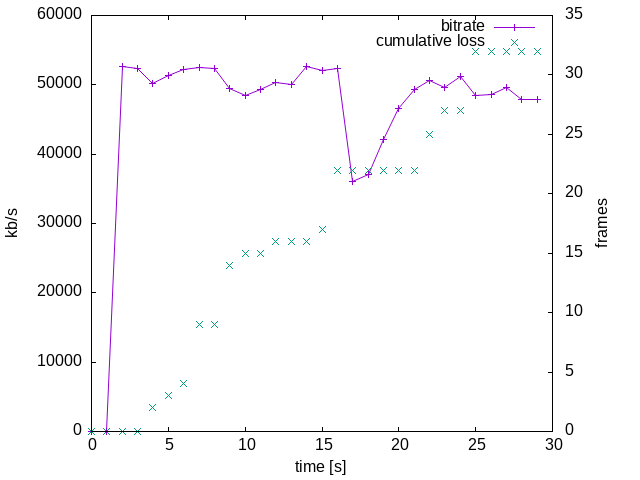
\includegraphics[width=0.5\linewidth]{plain_udp_client.png}
    \caption{UDP plain streaming - client}
    \label{fig:plain_udp_client}
\end{figure}

\subsection{Transcoded video streaming}


\begin{figure}[H]
    \centering
    \includegraphics[width=0.5\linewidth]{server_transcode_http_9000_lungo.pdf}
    \caption{HTTP 9Mbps -  Network bit-rate}
    \label{fig:server_transcode_http_9000_lungo}
\end{figure}

\begin{figure}[H]
    \centering
    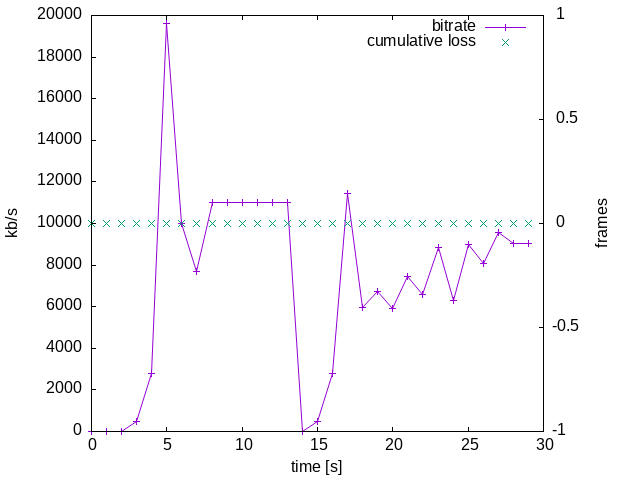
\includegraphics[width=0.5\linewidth]{transcode_http_9000_frame.png}
    \caption{Cumulative frame loss and bit-rate over TCP (9Mbps video transcoded)}
    \label{fig:transcode_http_9000_frame}
\end{figure}

\begin{figure}[H]
    \centering
    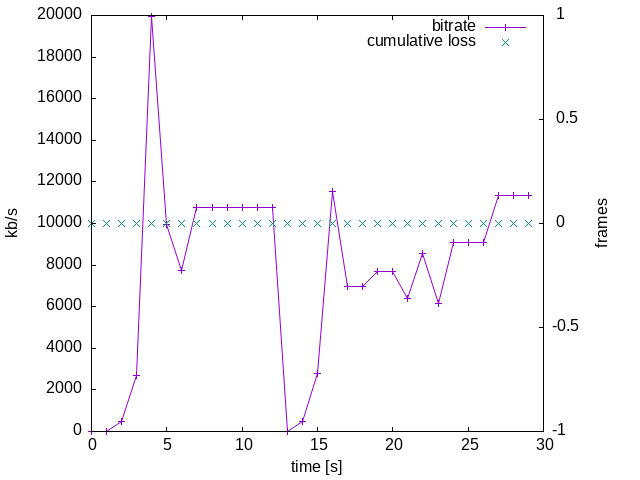
\includegraphics[width=0.5\linewidth]{loss_http_9000_frame.png}
    \caption{Cumulative frame loss and bit-rate over TCP (9Mbps video transcoded)}
    \label{fig:loss_http_9000_frame}
\end{figure}

\subsection{Impact of Packet Loss}
\begin{figure}[H]
    \centering
    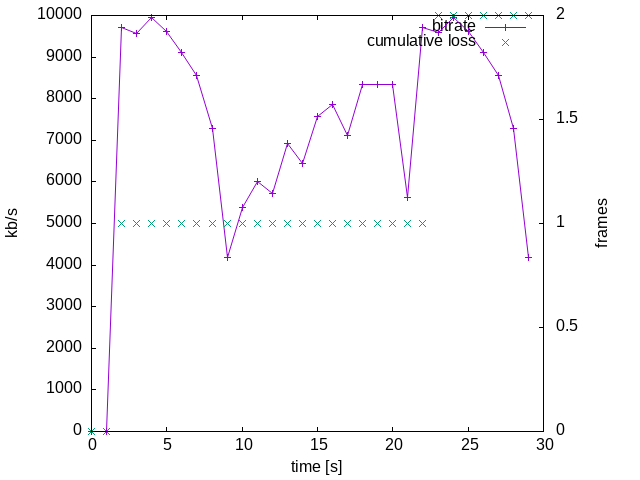
\includegraphics[width=0.5\linewidth]{transcode_udp_9000_frame.png}
    \caption{Cumulative frame loss and bit-rate over UDP (9Mbps video transcoded)}
    \label{fig:transcode_udp_9000_frame}
\end{figure}


\begin{figure}[H]
    \centering
    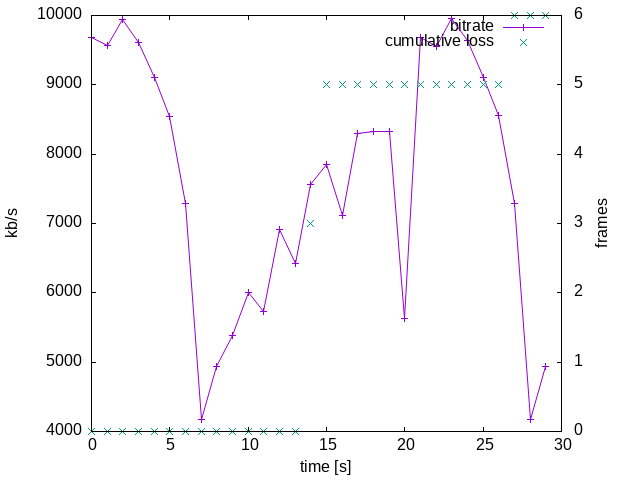
\includegraphics[width=0.5\linewidth]{loss_udp_9000_frame.png}
    \caption{Cumulative frame loss and bit-rate over UDP (9Mbps video transcoded)}
    \label{fig:loss_udp_9000_frame}
\end{figure}


\subsection{gap/length plot}
\begin{lstlisting}[language=python]
#!/bin/python3

import matplotlib.pyplot as plt
import csv
import os


def plain(r: str):
    dirs = os.listdir(r)

    for prot in dirs:
        with open(f"{r}/{prot}/stream.csv", 'r') as f:
            data = list(csv.reader((row.replace('\0', '') for row in f), delimiter=','))
            data = list(filter(lambda x: '1234' in x[8] or '8080' in x[7], data[1:]))

            time = [float(s[1]) for s in data]
            inter_packet_gap = [float(s[9]) for s in data]
            len = [float(s[5]) for s in data]
            
            plt.plot(time, inter_packet_gap, label=prot)

    plt.xlabel('Time (s)')
    plt.ylabel('Inter Packet Gap (s)')
    plt.legend()
    plt.title(label=r)
    plt.savefig(f"plain-gap.pdf", format='pdf')
    plt.show()

    for prot in dirs:
        with open(f"{r}/{prot}/stream.csv", 'r') as f:
            data = list(csv.reader((row.replace('\0', '') for row in f), delimiter=','))
            data = list(filter(lambda x: '1234' in x[8] or '8080' in x[7], data[1:]))

            time = [float(s[1]) for s in data]
            len = [float(s[5]) for s in data]
            
            plt.plot(time, len, label=prot)

    plt.xlabel('Time (s)')
    plt.ylabel('Packet Length (bytes)')
    plt.legend()
    plt.title(label=r)
    plt.savefig(f"plain-len.pdf", format='pdf')
    plt.show()


def transcode(r: str):
    dirs = os.listdir(r)

    for prot in dirs:
        vels = os.listdir(f"{r}/{prot}")

        for vel in vels:
            with open(f"{r}/{prot}/{vel}/stream.csv", 'r') as f:
                data = list(csv.reader((row.replace('\0', '') for row in f), delimiter=','))
                data = list(filter(lambda x: '1234' in x[8] or '8080' in x[7], data[1:]))

                time = [float(s[1]) for s in data]
                inter_packet_gap = [float(s[9]) for s in data]
                
                plt.plot(time, inter_packet_gap, label=f"{prot}@{vel}")
                    

    plt.xlabel('Time (s)')
    plt.ylabel('Inter Packet Gap (s)')
    plt.legend()
    plt.title(label=r)
    plt.savefig(f"transcode-gap.pdf", format='pdf')
    plt.show()

    for prot in dirs:
        vels = os.listdir(f"{r}/{prot}")

        for vel in vels:
            with open(f"{r}/{prot}/{vel}/stream.csv", 'r') as f:
                data = list(csv.reader((row.replace('\0', '') for row in f), delimiter=','))
                data = list(filter(lambda x: '1234' in x[8] or '8080' in x[7], data[1:]))

                time = [float(s[1]) for s in data]
                len = [float(s[5]) for s in data]
                
                plt.plot(time, len, label=f"{prot}@{vel}")
                    

    plt.xlabel('Time (s)')
    plt.ylabel('Packet Length (bytes)')
    plt.legend()
    plt.title(label=r)
    plt.savefig(f"transcode-len.pdf", format='pdf')
    plt.show()


plain('plain')
transcode('transcode')
\end{lstlisting}
\subsection{CPU usage plot}
\begin{lstlisting}[language=python]
#!/bin/python3

from subprocess import Popen, PIPE, run
import time
import matplotlib.pyplot as plt

def live(speeds: list[int], timeout: int, uni: list[int], multi: list[int]):
    for speed in speeds:
        vlc_uni = "cvlc /home/brendon/Downloads/jellyfish-50-mbps-hd-h264.mkv --sout='#transcode{vcodec=h264,acodec=mpga,vb=" + str(speed) + ",ab=128}:udp{mux=ts,dst=192.168.1.247:1234}' --loop"
        vlc_uni2 = "cvlc /home/brendon/Downloads/jellyfish-50-mbps-hd-h264.mkv --sout='#transcode{vcodec=h264,acodec=mpga,vb=" + str(speed) + ",ab=128}:udp{mux=ts,dst=192.168.1.55:1235}' --loop"
        
        cpu_uni = 0
        with Popen(f"/usr/bin/time -f %P timeout {timeout} {vlc_uni}", stderr=PIPE, shell=True) as p:
            with Popen(f"/usr/bin/time -f %P timeout {timeout} {vlc_uni2}", stderr=PIPE, shell=True) as p2:
                    cpu_uni += int(p.stderr.read().decode().split("\n")[-2][:-1])
                    cpu_uni += int(p2.stderr.read().decode().split("\n")[-2][:-1])

        print(f"Cpu uni usage: {cpu_uni}%")
        uni.append(cpu_uni)

        vlc_multi = "cvlc /home/brendon/Downloads/jellyfish-50-mbps-hd-h264.mkv --sout='#transcode{vcodec=h264,acodec=mpga,vb=" + str(speed) + ",ab=128}:udp{mux=ts,dst=224.0.0.1,sdp=sap,name=\"TestStream\"}' --loop"
        cpu_multi = 0
        with Popen(f"/usr/bin/time -f %P timeout {timeout} {vlc_multi}", stderr=PIPE, shell=True) as p:
            cpu_multi += int(p.stderr.read().decode().split("\n")[-2][:-1])

        print(f"Cpu multi usage: {cpu_multi}%")
        multi.append(cpu_multi)
    

def stored(speeds: list[int], timeout: int, uni: list[int], multi: list[int]):
    for speed in speeds:
        run("cvlc /home/brendon/Downloads/jellyfish-50-mbps-hd-h264.mkv vlc://quit --sout='#transcode{vcodec=h264,acodec=mpga,vb=" + str(speed) + ",ab=128}:file{mux=mp4,dst=jelly.mp4}'", shell=True)
        print("File created")
        
        vlc_uni = "cvlc ./jelly.mp4 --sout='#udp{mux=ts,dst=192.168.1.247:1234}' --loop"
        vlc_uni2 = "cvlc ./jelly.mp4 --sout='#udp{mux=ts,dst=192.168.1.55:1235}' --loop"
        
        cpu_uni = 0
        with Popen(f"/usr/bin/time -f %P timeout {timeout} {vlc_uni}", stderr=PIPE, shell=True) as p:
            with Popen(f"/usr/bin/time -f %P timeout {timeout} {vlc_uni2}", stderr=PIPE, shell=True) as p2:
                    cpu_uni += int(p.stderr.read().decode().split("\n")[-2][:-1])
                    cpu_uni += int(p2.stderr.read().decode().split("\n")[-2][:-1])

        print(f"Cpu uni usage: {cpu_uni}%")
        uni.append(cpu_uni)

        vlc_multi = "cvlc ./jelly.mp4 --sout='#udp{mux=ts,dst=224.0.0.1,sdp=sap,name=\"TestStream\"}' --loop"
        cpu_multi = 0
        with Popen(f"/usr/bin/time -f %P timeout {timeout} {vlc_multi}", stderr=PIPE, shell=True) as p:
            cpu_multi += int(p.stderr.read().decode().split("\n")[-2][:-1])

        print(f"Cpu multi usage: {cpu_multi}%")
        multi.append(cpu_multi)

def main():
    timeout = 20
    speeds = [1000, 2000, 5000, 10000]
    uni = []
    multi = []

    # live(speeds, timeout, uni, multi)
    stored(speeds, timeout, uni, multi)

    plt.plot(speeds, uni, label="Unicast")
    plt.plot(speeds, multi, label="Multicast")
    plt.ylabel("Cpu usage [%%]")
    plt.xlabel("Speed [Kb/s]")
    plt.legend()
    plt.show()
            

    

if __name__ == '__main__':
    main()
\end{lstlisting}


\end{document}